%! Author = user
%! Date = 27.12.2023

\documentclass[a4paper, 14pt]{article}
%\documentclass[draft]{article}

\usepackage[T2A]{fontenc}
\usepackage[utf8]{inputenc}
\usepackage[english, russian]{babel}
\usepackage[top = 2cm, bottom = 2cm, left = 2cm, right = 2cm]{geometry}
\usepackage{indentfirst}
\usepackage{xcolor}
\usepackage{hyperref}
\usepackage{gensymb}
\usepackage{pgfplots}
\usepackage{amsmath, amsfonts, amsthm, mathtools}
\usepackage{amssymb}
\usepackage{physics, multirow, float}
\usepackage{wrapfig, tabularx}
\usepackage{icomma} % Clever comma: 0,2 - number while 0, 2 - two numbers
\usepackage{tikz, standalone}
\usepackage{fancyhdr,fancybox}
\usepackage{lastpage}
\usepackage{booktabs}
\usepackage{listings}
\usepackage{lstmisc}
\usepackage{stmaryrd}

%\полуторный интервал
\onehalfspacing

\hypersetup
{   colorlinks = false,
    linkcolor = blue,
    pdftitle = {altissue3},
    pdfauthor = {Володин Максим},
    allcolors = [RGB]{010 090 200}
}

\graphicspath{{./images/}}
\DeclareGraphicsExtensions{.pdf,.png,.jpg}

\restylefloat{table}
\usetikzlibrary{external}

\mathtoolsset{showonlyrefs = true} % Numbers will appear only where \eqref{} in the text LINKED
\pagestyle{fancy}

\newcommand{\rot}{\mathop{\mathrm{rot}} \nolimits}

\fancyhf{}
\fancyhead[L]{Вопрос по выбору}
\fancyhead[R]{Волноводы}
\fancyfoot[L]{}
\fancyfoot[R]{\thepage /\pageref{LastPage}}

\pgfplotsset{compat=1.18}

\begin{document}
    \begin{titlepage}
        \begin{center}
        {\large МОСКОВСКИЙ ФИЗИКО-ТЕХНИЧЕСКИЙ ИНСТИТУТ \\ \vspace{5mm}
        НАЦИОНАЛЬНЫЙ ИССЛЕДОВАТЕЛЬСКИЙ УНИВЕРСИТЕТ \\ \vspace{5mm}
        КАФЕДРА ОБЩЕЙ ФИЗИКИ}
        \end{center}
        
        \begin{center}
        {\large}
        \end{center}
        
        \vspace{5cm}
        
        {\huge
            \begin{center}
            {\textbf{Вопрос по выбору}}
                \\
                Волноводы
            \end{center}
        }
        
        \vspace{2cm}
        
        \begin{flushright}
        {
            Володин Максим \\
            \vspace{2mm}
            Б02 -- 206к \\
            \vspace{2mm}
            Физтех-школа физики и исследований имени Ландау
        }
        \end{flushright}
        
        \tableofcontents \vspace{2.5cm}
        
        \begin{center}
            Долгопрудный \\
            24 января 2025 года
        \end{center}
    
    \end{titlepage}
    
    \section*{Историческая справка} \addcontentsline{toc}{section}{Историческая справка}
    
    Волновод — в общем случае — искусственный или естественный направляющий канал, в котором может распространяться
    волна.
    Он имеет поверхность идеального проводника и внутренность диэлектрика с $\varepsilon, \mu$
    
    По природе распространяющихся волн различают электромагнитные и акустические волноводы.
    Наиболее часто под термином «волновод» подразумеваются металлические трубки (Рис~\ref{1}), предназначенные для
    передачи энергии электромагнитных волн сверхвысокочастотных (СВЧ) и крайневысокочастотных (КВЧ) диапазонов (от МГц).
    По сути, волновод --- линия передачи, имеющая одну или несколько проводящих поверхностей, с поперечным сечением в
    виде замкнутого проводящего контура, охватывающего область распространения электромагнитной энергии
    
    \begin{figure}[h]
        \begin{center}
            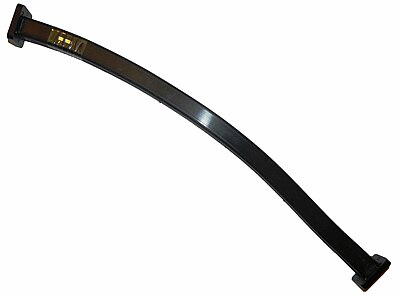
\includegraphics[width = 0.5 \textwidth]{1}
            \caption{Типичный волновод (изогнутый отрезок прямоугольного сечения с соединительными фланцами)}
            \label{1}
        \end{center}
    \end{figure}
    
    Впервые конструкция для передачи волн была предложена английским физиком Джозефом Джоном Томсоном (не путать с
    лордом Кельвиным) в 1893 году, а экспериментально проверили принцип этой конструкции всего годом позже.
    Первым математический анализ хода электромагнитных волн в металлическом цилиндре выполнил британский физик и
    механик Лорд Рэлей в 1897 году в процессе тщательного изучения звуковых волн (поверхностных акустических волн).
    Он опубликовал исследование в своём труде под названием «Теория звука».
    
    В дальнейшем, в 20-е годы $XX$ века началось изучение диэлектрических волноводов (в том числе и оптических волокон).
    Помимо Рэлея, изучением волноводов занимались математик Зоммерфельд, а также небезызвестный нидерландский физик
    Дебай.
    Фундаментальные исследования привели к тому, что с 1960-х волноводы стали привлекать к себе особое
    внимание
    
    \section*{(Не)экранированные волноводы} \addcontentsline{toc}{section}{(Не)экранированные и волноводы}
    
    По одной из классификаций, волноводы можно разделить на неэкранированные и экранированные.
    Экранированные волноводы имеют хорошо отражающие стенки для распространяющейся в нём волны, благодаря чему поток
    мощности волны сосредоточен внутри волновода.
    Как правило, такие волноводы выполнены в виде полых или заполненных диэлектриком (даже жидким).
    Поперечное сечение этих трубок имеет форму окружности, эллипса, прямоугольника, что связано с большей
    конструктивной простотой, хотя для специальных целей используются волноводы и с другими формами поперечного
    сечения (Рис~\ref{1}).
    Чтобы волна по мере распространения в волноводе не отражалась в обратном направлении, волновод выполняют
    регулярным: форма и размеры поперечного сечения, а также физические свойства материалов должны быть постоянны
    вдоль длины волновода (он должен быть однородным)
    
    К экранированным волноводам относят также акустические волноводы.
    Это трубы с достаточно жёсткими стенками, например, металлическими или пластмассовыми.
    В таких волноводах акустические колебания распространяются в газе, наполняющем волновод, как правило, в воздухе.
    
    \begin{figure}[h]
        \begin{center}
            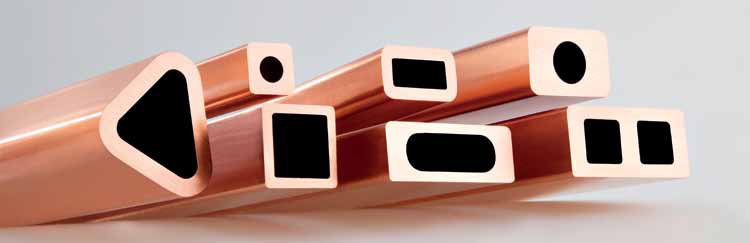
\includegraphics[width = 0.5 \textwidth]{waveguides}
            \caption{Волноводы разных сечений}
            \label{waveguides}
        \end{center}
    \end{figure}
    
    В открытых (неэкранированных) волноводах локализация поля обычно обусловлена явлением полного внутреннего
    отражения от границ раздела двух сред (в волноводах диэлектрических и оптоволоконных световодах), либо от
    областей с плавно изменяющимися параметрами среды (например, подводный звуковой канал, работающий на принципах
    рефракции (искривлении волны в среде) или градиентное оптоволокно).
    Поле локализуется преимущественно внутри специально предназначенной для этого области поперечного сечения
    волновода и быстро убывает за пределами этой области.
    Благодаря этому волна идёт по такому волноводу
    
    \section*{Математическое описание волновода} \addcontentsline{toc}{section}{Математическое описание волновода}
    
    Для волновода выполнены граничные условия
    \begin{gather*}
        E_{1\tau} = E_{2\tau} = E_\tau = 0 \\
        B_{1n} = B_{2n} = B_{3n} = 0
    \end{gather*}
    
    Запишем уравнения Максвелла для волновода
    \begin{gather*}
        \div E = 0 \\
        \div B = 0 \\
        \rot E = - \frac{1}{c} \frac{\partial B}{\partial t} \\
        \rot B = \frac{\varepsilon \mu}{c} \frac{\partial E}{\partial t}
    \end{gather*}
    
    Решение системы ищем в виде монохроматической волны: $E(x, y, z) = E_0 e^{-i(\omega t - kr)}$.
    В среде, в которой отсутствуют свободные заряды и токи проводимости, распространение электромагнитного поля
    описывается волновым уравнением
    \[ \frac{1}{v^2} \frac{\partial^2 E}{\partial t^2} = \frac{\partial^2 E}{\partial x^2} + \frac{\partial^2 E}
    {\partial y^2} + \frac{\partial^2 E}{\partial z^2} \]
    
    Здесь $v = \frac{c}{\sqrt{\varepsilon \mu}}$.
    Наша волна распространяется согласно гармоническому закону, поэтому более точно здесь будет уравнение Гельмгольца
    \[ \frac{\partial^2 E}{\partial x^2} + \frac{\partial^2 E}{\partial y^2} + \frac{\partial^2 E}{\partial z^2} =
    \frac{\omega^2}{c^2} E \]
    
    Для компонент вдоль $Oz$ уравнение принимает вид
    \[ \frac{\partial^2 E}{\partial x^2} + \frac{\partial^2 E}{\partial y^2} + \gamma^2 E_z = 0 \]
    
    Здесь введена новая переменна $\gamma^2 = \varepsilon \mu \frac{\omega^2}{c^2} - k^2$.
    Аналогичному уравнению удовлетворяет и вектор $B$.
    Однако оба этих вектора могут не удовлетворять нашим граничным условиям одновременно, но могут быть по отдельности.
    Для пояснения этого факта можно показать график гармонической функции с граничными условиями.
    Поэтому в волноводе существует несколько типов волн:
    
    \begin{itemize}
        \item $H-$волна, у которой $E_z = 0, B_n = 0$
        \item $E-$волна, у которой $B_z = 0, E_{z\tau} = 0$.
        \item Поперечная волна, у которой $E_z = 0, B_z = 0$.
        Такое возможно, лишь при условии $\gamma^2 = 0$
    \end{itemize}
    Итак, мы поняли, что решение уравнения существует не при всех $\gamma$, а лишь когда
    
    \begin{itemize}
        \item $\gamma^2 > 0$, иначе волны будут затухать в волноводе
        \item $k^2 = \varepsilon \mu \frac{\omega^2}{c^2} - \gamma^2 > 0$, то есть выполнено дисперсионное соотношение
    \end{itemize}
    
    Из дисперсионного соотношения можно найти минимальную частоту, с которой распространяются волны в волноводе --
    $\omega_{cr}$, поставив знак равенства в дисперсионное соотношение
    
    Таким образом, волновое число $k = \frac{\varepsilon \mu}{c} \sqrt{\omega^2 - \omega^2_{cr}}$ всегда
    действительно, а фазовая и групповая (скорость переноса энергии) находятся как $v_{ph} =
    \frac{\omega}{k}, v_{gr} = \frac{c^2}{\varepsilon \nu} \frac{1}{v_{ph}}$
    
    \section*{Волна в прямоугольном волноводе} \addcontentsline{toc}{section}{Волна в прямоугольном волноводе}
    
    Рассмотрим бегущую в волноводе $H-$волну: $E = E_0 (x, y) e^{-i(\omega t - k_z z)}$ с решением
    \begin{gather*}
        E_x = E_{0x} \cos(k_x x) \sin(k_y y) e^{-i(\omega t - k_z z)} \\
        E_y = E_{0y} \sin(k_x x) \cos(k_y y) e^{-i(\omega t - k_z z)}
        \label{eq:}
    \end{gather*}
    
    Система удовлетворит граничным условиям, если $k_x = l \frac{\pi}{a}, k_y = p \frac{\pi}{b}$.
    Тогда
    \[ \frac{\omega^2}{c^2} = k^2_x + k^2_y + k^2_z = \left(l \frac{\pi}{a}\right)^2 + \left(p \frac{\pi}{b}\right)^2 +
    k^2_z \]
    
    Оба параметра не могут нулями, иначе $E \equiv 0$.
    Если $a > b$ критическая частота тогда будет $\omega_{cr} = \frac{\pi c}{a}$
    
    \begin{figure}[h]
        \begin{center}
            \begin{minipage}[h]{0.74\linewidth}
                \centering
                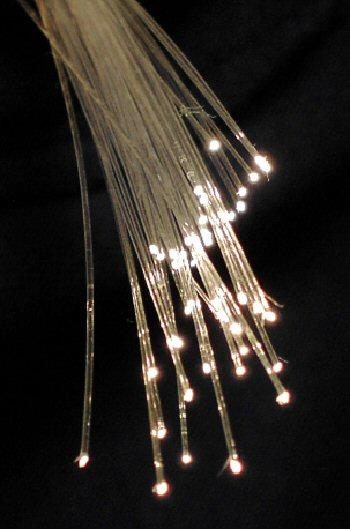
\includegraphics[width = 0.47 \textwidth]{fibreoptic}
                \caption{Пучок оптических волокон}
                \label{fig:fibreoptic}
            \end{minipage}
        \end{center}
    \end{figure}
    
    \section*{Применение волноводов} \addcontentsline{toc}{section}{Применение волноводов}
    
    Волноводы нашли себе широкое применение
    
    \begin{itemize}
        \item В бытовой микроволновой печи через полый металлический радиоволновод энергия от магнетрона, являющегося
        источником электромагнитных волн, поступает в камеру для разогрева
        \item Акустические волноводы ранее широко применялись на судах и кораблях в качестве переговорных труб.
        Сейчас они дублируют электронные переговорные устройства при их отказе.
        \item Волноводы и, в частности, оптоволокно (Рис~\ref{fig:fibreoptic}) используют для передачи данных и
        обеспечения связи.
        Применяется в сетях кабельного телевидения и для высокоскоростного доступа в Интернет
    \end{itemize}
    
    \phantomsection \addcontentsline{toc}{section}{Список литературы}
    \begin{thebibliography}{}
        
        \bibitem{1} Лабораторный практикум по общей физике: учебное пособие.
        В трёх томах.~Т.~2.~Оптика / А.~В.~Максимычев, Д.~А.~Александров, Н.~С.~Берюлёва и др.;
        под ред.~А.~В.~Максимычева.~— М.~: МФТИ, 2014.~— 446 с
        
        \bibitem{2} \href{https://textarchive.ru/c-2236776.html}{Банк научно-популярных статей textarchive.
        Статья 'Особенности расчёта устройств СВЧ' под авторством Д.И. Воскресенского}.
        Режим доступа -- свободный.
        Дата обращения -- 23.01.2025.
        
        \bibitem{3} [Источник изображений] \href{https://ru.wikipedia.org/wiki/Оптическое_волокно}
        {Интернет-энциклопедия}.
        Режим доступа -- свободный.
        Дата обращения -- 23.01.2025.
    
    \end{thebibliography}

\end{document}